% Options for packages loaded elsewhere
\PassOptionsToPackage{unicode}{hyperref}
\PassOptionsToPackage{hyphens}{url}
%
\documentclass[
]{book}
\usepackage{amsmath,amssymb}
\usepackage{iftex}
\ifPDFTeX
  \usepackage[T1]{fontenc}
  \usepackage[utf8]{inputenc}
  \usepackage{textcomp} % provide euro and other symbols
\else % if luatex or xetex
  \usepackage{unicode-math} % this also loads fontspec
  \defaultfontfeatures{Scale=MatchLowercase}
  \defaultfontfeatures[\rmfamily]{Ligatures=TeX,Scale=1}
\fi
\usepackage{lmodern}
\ifPDFTeX\else
  % xetex/luatex font selection
\fi
% Use upquote if available, for straight quotes in verbatim environments
\IfFileExists{upquote.sty}{\usepackage{upquote}}{}
\IfFileExists{microtype.sty}{% use microtype if available
  \usepackage[]{microtype}
  \UseMicrotypeSet[protrusion]{basicmath} % disable protrusion for tt fonts
}{}
\makeatletter
\@ifundefined{KOMAClassName}{% if non-KOMA class
  \IfFileExists{parskip.sty}{%
    \usepackage{parskip}
  }{% else
    \setlength{\parindent}{0pt}
    \setlength{\parskip}{6pt plus 2pt minus 1pt}}
}{% if KOMA class
  \KOMAoptions{parskip=half}}
\makeatother
\usepackage{xcolor}
\usepackage{longtable,booktabs,array}
\usepackage{calc} % for calculating minipage widths
% Correct order of tables after \paragraph or \subparagraph
\usepackage{etoolbox}
\makeatletter
\patchcmd\longtable{\par}{\if@noskipsec\mbox{}\fi\par}{}{}
\makeatother
% Allow footnotes in longtable head/foot
\IfFileExists{footnotehyper.sty}{\usepackage{footnotehyper}}{\usepackage{footnote}}
\makesavenoteenv{longtable}
\usepackage{graphicx}
\makeatletter
\def\maxwidth{\ifdim\Gin@nat@width>\linewidth\linewidth\else\Gin@nat@width\fi}
\def\maxheight{\ifdim\Gin@nat@height>\textheight\textheight\else\Gin@nat@height\fi}
\makeatother
% Scale images if necessary, so that they will not overflow the page
% margins by default, and it is still possible to overwrite the defaults
% using explicit options in \includegraphics[width, height, ...]{}
\setkeys{Gin}{width=\maxwidth,height=\maxheight,keepaspectratio}
% Set default figure placement to htbp
\makeatletter
\def\fps@figure{htbp}
\makeatother
\setlength{\emergencystretch}{3em} % prevent overfull lines
\providecommand{\tightlist}{%
  \setlength{\itemsep}{0pt}\setlength{\parskip}{0pt}}
\setcounter{secnumdepth}{5}
\usepackage{booktabs}
\ifLuaTeX
  \usepackage{selnolig}  % disable illegal ligatures
\fi
\usepackage[]{natbib}
\bibliographystyle{plainnat}
\IfFileExists{bookmark.sty}{\usepackage{bookmark}}{\usepackage{hyperref}}
\IfFileExists{xurl.sty}{\usepackage{xurl}}{} % add URL line breaks if available
\urlstyle{same}
\hypersetup{
  pdftitle={LPS 30 Discussion Notes},
  pdfauthor={Ryan Chen},
  hidelinks,
  pdfcreator={LaTeX via pandoc}}

\title{LPS 30 Discussion Notes}
\author{Ryan Chen}
\date{2024-02-01}

\begin{document}
\maketitle

{
\setcounter{tocdepth}{1}
\tableofcontents
}
\hypertarget{about}{%
\chapter{About}\label{about}}

These are notes for Ryan Chen's LPS 30 Discussion Sections (Monday 1-2 p.m. and 4-5 p.m.). These notes summarize the material covered in discussion. For this course, it primarily consists of definitions, exercises and worked out solutions to exercises. These notes are intended for students who want to review course material and students which miss discussion for whatever reason. They are not a replacement for attending discussion section.

\hypertarget{propositions-and-validity}{%
\chapter{Propositions and Validity}\label{propositions-and-validity}}

{[}I have tried to include as much detail as possible in this week's notes. This is because we did not have discussion in week 2, and so this is meant to be a sort of replacement. Future weeks may be more sparse.{]}

\hypertarget{propositions}{%
\section{Propositions}\label{propositions}}

What is a proposition? According to the slides, \emph{a proposition is a thing we could believe or disbelieve}. Importantly, propositions are expressed by sentences (propositions are not sentences themselves). More importantly, propositions are expressed by a certain kind of sentence: declarative sentences. So, the question of identifying which sentences express propositions is really a question of identifying the declarative sentences.

There are a number of ways to test whether or not a sentence is a declarative sentence. Here, is one given in lecture: (Step One) take the sentence you want to test and stick ``I believe that\ldots{}'' in front of it. (Step Two) If the result of sticking ``I believe that\ldots{}'' in front of the sentence still makes sense, then the original sentence expresses a proposition.

\textbf{{[}Example One{]}} Consider the sentence ``It is raining''. (Step One) To test this sentence, I stick ``I believe that\ldots{}'' in front of it. So, I get, ``I believe that it is raining''. (Step Two) Now, I ask myself, does it make sense to say ``I believe that it is raining''? It does. Therefore, ``It is raining'' expresses a proposition.

\textbf{{[}Example Two{]}} Consider the sentence ``Coffee is tasty''. (Step One) To test this sentence, I stick ``I believe that\ldots{}'' in front of it. So, I get, ``I believe that coffee is tasty''. (Step Two) Now, I ask myself, does it make sense to say ``I believe that coffee is tasty''? It does. Therefore, ``Coffee is tasty'' expresses a proposition. (Note: most people think that whether or not coffee is tasty is a matter of personal preference. Nonetheless, the sentence ``coffee is tasty'' still expresses a proposition. Just because a sentence expresses a proposition the truth (or falsity) of which depends on one's own taste, does not mean that that sentence does not express a proposition.)

\textbf{{[}Example Three{]}} Consider the sentence ``Please close the door''. (Step One) To test this sentence, I stick ``I believe that\ldots{}'' in front of it. So, I get, ``I believe that please close the door''. (Step Two) Now, I ask myself, does it make sense to say ``I believe that please close the door''. It does not. Therefore, ``Please close the door'' does not express a proposition.

From now on, I will be less wordy on these examples:

\textbf{{[}Example Four{]}} Consider the sentence ``Earth is the eighth planet in the solar system''. (Step One) ``I believe that Earth is the eighth planet in the solar system''. (Step Two) Does this make sense? Yes. Therefore, ``Earth is the eighth planet in the solar system'' expresses a proposition. (Note: Earth is of course not the eighth planet in the solar system. Nonetheless, ``Earth is the eighth planet in the solar system'' expresses a proposition. Just because a sentence is false does not mean it does not express a proposition.)

\textbf{{[}Example Five{]}} Consider the sentence ``I believe that it will rain tomorrow''. (Step One) ``I believe that I believe that it will rain tomorrow''. (Step Two) Does this make sense? Yeah (If this is not obvious to you, replace the original sentence with ``John believes that it will remain tomorrow''; it should be clear to you that ``I believe that John believes that it will remain tomorrow'' makes sense to say. Now the original example should sound better).

Now that we know what a proposition is, we can define what an argument is. \emph{An argument is a list of propositions}. We call the last proposition, the \emph{conclusion} of the argument. We call all the other propositions, the \emph{premises}.

\hypertarget{validity}{%
\section{Validity}\label{validity}}

We want to know which arguments are good arguments. To do so, we use the notion of validity. \emph{An argument is valid if and only if if the premises are true then the conclusion must be true}. I prefer this alternative, but equivalent definition: \emph{An argument is valid if and only if it is impossible for the premises to be true and the conclusion false}.

The definition tells us how to assess whether or not an argument is valid or not. (Step One) First, we \emph{suppose} that the premises of the argument are true. Note that this does not mean that the premises are in fact true. You suppose that the premises are true for the sake of argument. (Step Two) Now you ask, whether or not the conclusion \emph{must} be true given the supposition that you make in step one (i.e., under the (potentially) hypothetical situation where the premises are true).

\textbf{{[}Example One{]}} Consider the argument:

\begin{enumerate}
\def\labelenumi{\arabic{enumi}.}
\tightlist
\item
  All cats are dogs.
\item
  All dogs are books.
\item
  Therefore, all cats are books.
\end{enumerate}

(Step One) Let us suppose that all cats are dogs and all dogs are books. That is, we are under the hypothetical situation in which all cats are dogs and all dogs are books (never mind what such a universe would look like, just suppose they are true!). (Step Two) Under such a supposition, does it \emph{necessarily} follow that all cats are books? Yes! For now, I hope you share my intuition on this matter; as the course progress, we will develop more and more tools to help you see why this conclusion necessarily follows. (Note: we are starting this course with propositional logic. It turns out that in propositional logic, there is no obvious way to represent the argument just given as valid. So look forward to predicate logic where we can represent such arguments)

\textbf{{[}Example Two{]}} Consider the argument:

\begin{enumerate}
\def\labelenumi{\arabic{enumi}.}
\tightlist
\item
  If Ryan is writing these notes at 2 am then Ryan will wake up tired in the morning.
\item
  If Ryan will wake up tired in the morning then Ryan will get coffee in the morning.
\item
  Ryan is writing these notes at 2 am.
\item
  Therefore, Ryan will get coffee in the morning.
\end{enumerate}

(Step One) Let us suppose that all the premises are true. (Step Two) Since premise three tells us that Ryan is writing these notes at 2 am then when we combine that fact with premise one, it seems that we must conclude that Ryan will wake up tired in the morning. Well, since Ryan will wake up tired in the morning, then we can combine that fact with premise two, and we must conclude that Ryan will get coffee in the morning. This shows that the argument is valid. Here, I tried to use a bit of reasoning to show you why you must arrive at the conclusion.

\textbf{{[}Example Three{]}} Consider the argument:

\begin{enumerate}
\def\labelenumi{\arabic{enumi}.}
\tightlist
\item
  If Ryan is mortal then Ryan will one day pass away.
\item
  Ryan is mortal.
\item
  Therefore, Ryan is a PhD student
\end{enumerate}

(Step One) Let us suppose that all the premises are true. (Step Two) You should ask yourself, can it be the case that premise 1 and 2 are true while premise 3 false? It certainly seems so. I could have not pursued graduate school and pursued some other career. Nothing about the premises seems to necessitate the conclusion that Ryan is a PhD student. Hence, the argument is invalid (Note: the premises and the conclusion of this argument are true, yet the argument is invalid. There is a general lesson here. Just because an argument has true premises and a true conclusion does not mean that it is valid)

From now on, I will skip writing out step one.

\textbf{{[}Example Four{]}} Consider the argument:

\begin{enumerate}
\def\labelenumi{\arabic{enumi}.}
\tightlist
\item
  Ryan prefers cats to dogs.
\item
  If water is H2O then copper conducts electricity.
\item
  Copper does not conduct electricity.
\item
  Therefore, water is not H2O.
\end{enumerate}

(Step Two) Since, by premise 3, Copper does not conduct electricity, it cannot be the case that water is H2O. Why? Here's a bit of reasoning: If water was H2O then by premise 2 I would be forced to conclude that copper conducts electrity. By premise 3, it is not the case that copper conducts electricity. Well it cannot be the case that copper conducts electricity and it does not conduct electricity; that is just absurd! We have to think to ourselves, is there a way that both premise 2 and premise 3 are true concurrently? Yes! it must then be the case that water is not H2O. Now I am not forced to conclude that copper conducts electricity and so all the premises can remain true at the same time. Therefore, the argument is valid. (Note: notice here that premise 1 is never used. All that is needed to get the conclusion are premises 2 and 3. This tells us something important: an argument may have irrelevant premises and still be valid)

\textbf{{[}Example Five{]}} Consider the argument:

\begin{enumerate}
\def\labelenumi{\arabic{enumi}.}
\tightlist
\item
  Squirtle ate food at 4 pm four days ago.
\item
  Squirtle ate food at 4 pm three days ago.
\item
  Squirtle ate food at 4 pm two days ago.
\item
  Squirtle ate food at 4 pm yesterday.
\item
  Therefore, Squirtle will eat food at 4 pm today.
\end{enumerate}

(Step Two) Can it be the case that even if I accept all the premises, the conclusion is false? Yes! Squirtle might be stopped from eating food at 4 pm; maybe, Squirtle just is not hungry. Hence, this argument is invalid. (Note: notice that there is still something compelling about this argument. This sort of argument is called an inductive argument, and while invalid, they seem to be used all the time. Saying why such arguments are good has been a major problem for philosophers for centuries).

\textbf{{[}Example Six{]}} Consider the argument:

\begin{enumerate}
\def\labelenumi{\arabic{enumi}.}
\tightlist
\item
  Tom went to the mall and Jerry followed after Tom.
\item
  Therefore, Jerry followed after Tom.
\end{enumerate}

(Step Two) If Tom went to the mall and Jerry followed after Tom is true then it simply just followed that Jerry followed after Tom! Hence, this argument is valid.

\textbf{{[}Example Seven{]}} Consider the argument:

\begin{enumerate}
\def\labelenumi{\arabic{enumi}.}
\tightlist
\item
  Either it is the case that Tom went to the mall or Jerry went to the mall.
\item
  Therefore, Tom went to the mall.
\end{enumerate}

(Step Two) Well, just because we suppose that either Tom went to the mall or Jerry went to the mall does not mean that it must follow that Tom went to the mall. It could be the case that Jerry went to the mall and Tom did not go to the mall. Under that possibility, premise 1 would still be true but the conclusion would be false. Therefore, the argument is invalid.

\textbf{{[}Example Eight{]}} Consider the argument:

\begin{enumerate}
\def\labelenumi{\arabic{enumi}.}
\tightlist
\item
  If it is raining then everyone wins the lottery.
\item
  Everyone wins the lottery.
\item
  Therefore, it is raining.
\end{enumerate}

(Step Two) Well, just because everyone won the lottery does not mean that it is raining. What premise 1 tells us is that if it is raining then we must conclude that everyone wins the lottery. But it does not tell us that it is in fact the case that it is raining. It is perfectly possible for it to be sunny and clear out and everyone wins the lottery. In which case, all the premises are true and the conclusion false. Therefore, the argument is invalid.

Next week, we will return to a couple more arguments.

\hypertarget{soundness}{%
\section{Soundness}\label{soundness}}

\emph{An argument is sound if and only if it is valid and the premises are actually true}. Notice the difference between soundness and validity. Validity requires that \textbf{if} the premises are true then the conclusion must be true. That is, it requires that under the hypothetical situation that the premises are true then the conclusion must be true. Soundness requires that the premises are in fact true.

I will not say more about soundness here. Of course, you are welcome to ask questions in discussion or office hours. I think it is beneficial to sit down and think through the differences between the definitions of validity and soundness and the relations that they bear to one another (your homework makes you think about this).

\hypertarget{argument-forms}{%
\section{Argument Forms}\label{argument-forms}}

To get an argument form, you look at a given argument, look for sentences which express propositions in them and replace those sentences with letters like \(A,B,C,\ldots\). Note that you are allowed to replace parts of sentences which express propositions with letters as well.

\textbf{{[}Example One{]}} Consider the argument:

\begin{enumerate}
\def\labelenumi{\arabic{enumi}.}
\tightlist
\item
  Either the world is round or the sun is round.
\item
  If the world is round then the sea is wet.
\item
  The sun is round.
\item
  Therefore, the world is round.
\end{enumerate}

Notice that in premise 1, the sentence ``either the world is round or the sun is round'' has two parts ``the world is round'' and ``the sun is round'' which themselves express propositions. Hence, we can represent this premise as ``Either \(A\) or \(B\)'' where \(A\)=the world is round and \(B\)=the sun is round. Again, in premise 2, the sentence ``If the world is round then the sea is wet'' has two parts ``the world is round'' and ``the sea is wet'' which express propositions. We can represent this premise with ``if \(A\) then \(C\)'' where it continues to be the case that \(A\)=the world is round and \(C\)=the sea is wet. The other two premises are straightforward and we get:

\begin{enumerate}
\def\labelenumi{\arabic{enumi}.}
\tightlist
\item
  Either \(A\) or \(B\)
\item
  If \(A\) then \(C\)
\item
  \(B\)
\item
  Therefore, \(A\)
\end{enumerate}

Some argument forms are valid. They are not valid in the same sense that an argument is valid. Instead, \emph{an argument form is valid if and only if every instance of that argument form is valid}.

That is, when we are given an argument form we are given something that looks like an argument but with a bunch of letters like \(A,B,C,D,E,\ldots\) (just see the previous example). To get an instance of that argument form, you replace all these letters with sentences (which express propositions). So, continuing with our example:

\begin{enumerate}
\def\labelenumi{\arabic{enumi}.}
\tightlist
\item
  Either \(A\) or \(B\)
\item
  If \(A\) then \(C\)
\item
  \(B\)
\item
  Therefore, \(A\)
\end{enumerate}

We see that there are three letters \(A\), \(B\), and \(C\) which appear in that argument form. To get an instance of this form, let \(A\)=Tom is funny, let \(B\)=Tom is hungry, and let \(C\)=Jerry is tired (these are just random sentences that I have chosen). Then putting these sentences into the argument form yields:

\begin{enumerate}
\def\labelenumi{\arabic{enumi}.}
\tightlist
\item
  Either Tom is funny or Tom is hungry.
\item
  If Tom is funny then Jerry is tired.
\item
  Tom is hungry.
\item
  Therefore, Tom is funny.
\end{enumerate}

I leave it to you to verify that this argument is in fact invalid. Since, the argument form has an instance which is invalid, the argument form itself is invalid.

What is an example of a valid argument form? Here are two examples:

\textbf{{[}Example One{]}} Consider the argument form:

\begin{enumerate}
\def\labelenumi{\arabic{enumi}.}
\tightlist
\item
  If \(A\) then \(B\)
\item
  \(A\)
\item
  Therefore, \(B\)
\end{enumerate}

\textbf{{[}Example Two{]}} Consider the argument form:

\begin{enumerate}
\def\labelenumi{\arabic{enumi}.}
\tightlist
\item
  \(A\) and \(B\)
\item
  Therefore, \(B\)
\end{enumerate}

How do we check? At this point in this course we do not have the means to verify that all instances of this argument form are valid. The problem is that to check whether or not an argument form is valid, we need to answer the following question: if I substitute in any sentences (which express propositions) for \(A\) and \(B\), then is the resulting argument valid? The crucial bit here is that you need to check for \emph{any} sentence and there are an infinite number of possible sentences in English which express propositions. It would take you an awfully long time to go through an infinite number of sentences.

Thankfully, checking for invalid argument forms is doable. Here is another example (now with explicity steps):

\textbf{{[}Example Three{]}} Consider the argument form:

\begin{enumerate}
\def\labelenumi{\arabic{enumi}.}
\tightlist
\item
  \(A\)
\item
  If \(C\) then \(A\) and \(B\)
\item
  Therefore, \(C\)
\end{enumerate}

To check that this is an invalid argument form you need to come up with sentences (which express propositions) such that if you substitute those sentences in, the resulting argument is invalid. So, (Step One), come up with as many sentences as there are different letters in the argument form. Here there are three letters, \(A\), \(B\) and \(C\), so we need three sentences. Let us use: \(A\)=``Bob is funny'', \(B\)=``Jerry is silly'', and \(C\)=``It is hot out today''. Next, (Step Two), we need to substitute these into the argument form:

\begin{enumerate}
\def\labelenumi{\arabic{enumi}.}
\tightlist
\item
  Bob is funny.
\item
  If it is hot out today then Bob is funny and Jerry is silly.
\item
  Therefore, it is hot out today.
\end{enumerate}

Now, (Step Three), check for validity. So, now you need to follow the steps to check for validity. Hopefully, at this point you can check that this argument is invalid.

\hypertarget{translation}{%
\chapter{Translation}\label{translation}}

This week in discussion we mainly practiced translation problems. There are a couple key skills to learn here:

\begin{enumerate}
\def\labelenumi{\arabic{enumi}.}
\tightlist
\item
  Given a English sentence which expresses a proposition, you should be able to translate it into propositional logic.
\item
  Given an argument, you should be able to translate it into propositional logic.
\item
  Given a string of symbols, you should be able to evaluate whether or not it is a formula in propositional logic.
\item
  Given a formula in propositional logic, you should be able to translate it back into English.
\end{enumerate}

We only practiced the first skill in discussion. The second skill should follow immediately from knowing how to do the first. We will touch more on the third skill in week 4, but also see the Translation and Language Slides on canvas, starting from slide 25. Finally, skill 4 was not covered, so I will give an example of this at the end of these notes.

\hypertarget{translating-from-english-to-propositional-logic}{%
\section{Translating from English to Propositional Logic}\label{translating-from-english-to-propositional-logic}}

In a question where you are asked to translate an English sentence or an argument into propositional logic, you do the following:

\begin{itemize}
\tightlist
\item
  (Step One) Provide a dictionary. That is, for every part of a sentence that expresses a proposition in the sentence, assign it a unique lower-case letter. {[}NOTE: Sometimes this involves first rewriting the sentence, so that it is clear what all the sentence parts are. More on this in the example{]}
\item
  (Step Two) Go through that sentence and replace all the parts of the sentence with their corresponding letters according to the dictionary.
\item
  (Step Three) Go through the result of step two and examine all the English expressions which remain. If any of the left-over expressions correspond to a propositional connective, then look for the propositional letters which the connective is binding together. Then, following the rules for constructing formulas in propositional logic, replace the expression, with the symbol corresponding to the propositional connective.
\end{itemize}

Note that these steps give you the general strategy that you should use when translating. Sometimes, you may need to still bring your intuitions to the table when doing this sort of exercise.

{[}Example One{]} Consider the sentence: ``If Tom went to the mall then Jerry fell down the stairs''. (Step One) We see here that ``Tom went to the mall'' and ``Jerry fell down the stairs'' are sentences which express propositions. These are the parts of the larger sentence ``If Tom went to the mall then Jerry fell down the stairs'' which we want to assign unique letters. So, let \(t\)=Tom went to the mall and \(j\)=Jerry fell down the stairs. (Step Two) When we replace the parts of the sentences with the propositional letters, we get ``If \(t\) then \(j\)''. (Step Three) Now, we see that the phrase is of the form ``If\(\ldots\) then\(\ldots\)'' which corresponds to the propositional connective \(\supset\). We also note that the conditional is operating on \(t\) and \(j\) with \(t\) being the antecedent and \(j\) being the consequent. Hence, following the rules for how to build formulas in propositional logic, we get \((t \supset j)\).

{[}Example Two{]} Consider the sentence: ``Tom and Jerry went to the mall''. (Step One) Here, we can first rewrite the sentence to reveal its underlying structure. ``Tom and Jerry went to the mall'' can be rewritten as ``Tom went to the mall and Jerry went to the mall'' (this trick does not always work). Now, we can provide a dictionary: \(t\)=Tom went to the mall, \(j\)=Jerry went to the mall. (Step Two) Replacing the sentences with their propositional letters, we get ``\(t\) and \(j\)''. (Step Three) We note that this is of the form ``\(\ldots\)and\(\ldots\)'' and that it binds together, \(t\) and \(j\), so we get \((t \& j)\).

{[}Example Three{]} I go a bit quicker in this example. Consider the sentence: ``If Tom went to the mall and Jerry went to the mall then Adam went to the mall''. (Step One) Dictionary: \(t\)=Tom went to the mall, \(j\)=Jerry went to the mall, and \(a\)=Adam went to the mall. (Step Two) Replacing the sentences with their propositional letters, we get ``If \(t\) and \(j\) then \(a\)''. (Step Three) Now here is where we need to be a bit careful.We need to note that the ``If\(\ldots\)then\(\ldots\)'' clause has as its antecedent ``\(t\) and \(j\)'' and its consequent \(a\).''\(t\) and \(j\)'' just translates into \((t \& j)\) (see Example Two). So, we end up with ``If \((t \& j)\) then \(a\)''. This just translates into \(((t \& j) \supset a)\) (see Example One).

\hypertarget{practice-problems}{%
\section{Practice Problems}\label{practice-problems}}

Here are the questions in section (A) and section (B) which we worked on in discussion section. If you have not tried doing them, I recommend trying to translate them before looking at the solutions:

\begin{itemize}
\tightlist
\item
  (A1) If Mary is the sister of Jane then Jane is Bill's aunt.
\item
  (A2) Either Jones bluffed his hand or Jones is crazy.
\item
  (A3) Neither Jones nor Sally were happy with the colour blue.
\item
  (A4) Tables are solid if and only if books are readable.
\item
  (A5) Tom went to the mall and Jerry went to bed.
\item
  (A6) Tom went to the mall but Jerry went to bed.
\item
  (A7) If Jesse lies and Frank cheats then the Thagard's are crooks.
\item
  (A8) If Jesse lies then if Frank cheats then the Thagard's are crooks.
\item
  (A9) If Jesse and Frank are crooks then either George is a crook or the sky is falling.
\item
  (B1) If Alfred is a spy then Rudolf is breaking the law.
\item
  (B2) Alfred is a spy only if Rudolf is breaking the law.
\item
  (B3) Alfred is a spy if Rudolf is breaking the law.
\item
  (B4) Alfred is a spy unless Rudolf is breaking the law.
\item
  (B5) It will be hot out tomorrow and quite damp, unless the eastern winds pick up today.
\item
  (B6) Debra will not leave until the others do, but, only if Meredith is in the office.
\item
  (B7) If the ball is red then Ash won the competition unless the second ball drawn is blue.
\item
  (B8) If Lee wants it, Lee can get it, but Lee should not blame Sarah if Sarah gets in trouble.
\item
  (B9) If Justin's heart stops beating then Justin will live if the doctors apply electric shock.
\end{itemize}

\hypertarget{practice-problem-solutions}{%
\section{Practice Problem Solutions}\label{practice-problem-solutions}}

Here are the solutions. If it is obvious, then I leave the dictionary out:

\begin{itemize}
\tightlist
\item
  (A1) \((m \supset j)\)
\item
  (A2) Dictionary: \(j\)=Jones bluffed his hand, \(c\)=Jones is crazy. Answer: \((j \lor c)\)
\item
  (A3) \(\sim(j \lor s)\) (it is equally acceptable to write \((\sim j \& \sim s)\))
\item
  (A4) \((t \equiv b)\)
\item
  (A5) \((t \& j)\)
\item
  (A6) \((t \& j)\) {[}NOTE: A5 and A6 have the same answer{]}
\item
  (A7) \(((j \& f) \supset t)\)
\item
  (A8) \((j \supset (f \supset t))\)
\item
  (A9) \(((j \& f) \supset (g \lor s))\)
\item
  (B1) \((a \supset r)\)
\item
  (B2) \((a \supset r)\) {[}NOTE: B1 and B2 have the same answer{]}
\item
  (B3) \((r \supset a)\)
\item
  (B4) \((\sim r\supset a)\)
\item
  (B5) \((\sim e \supset (h \& d))\)
\item
  (B6) This one is trickier than I thought and so I won't provde an answer here. You won't get a question this tricky.
\item
  (B7) Here are two possible answers: \((\sim b \supset (r \supset a))\) and \((r \supset (\sim b \supset a))\)
\item
  (B8) Dictionary: \(w\)=Lee wants it, \(g\)=Lee gets it, \(b\)=Lee should blame Sarah, \(t\)=Sarah gets in trouble. Answer: \(((w \supset g) \& (t \supset \sim b))\)
\item
  (B9) \((h \supset (e \supset l))\)
\end{itemize}

\hypertarget{translating-from-propositional-logic-to-english}{%
\section{Translating from Propositional Logic to English}\label{translating-from-propositional-logic-to-english}}

{[}Example{]} Consider the following dictionary \(a\)=Albert is funny, \(b\)=Bart is smart, and \(c\)=Cassandra is athletic. Then consider the following formula \((\sim a \supset (b \& c))\). To translate this back into English, let us first translate the connectives back into English. Let us start with the \(\supset\), so we get ``If \(\sim a\) then \((b \& c)\)''. Now we translate the \(\sim\) to get, ``If it is not the case that \(a\) then \((b \& c)\)''. Next is the \(\&\) to get, ``If it is not the case that \(a\) then \(b\) and \(c\)''. Finally, we plug the sentences back in: ``If it is not the case that Albert is funny then Bart is smart and Cassandra is athletic''. Sometimes, if you follow this sort of procedure, if does not make sense. You may have to move words around in order to make it make sense.

\hypertarget{truth-tables}{%
\chapter{Truth Tables}\label{truth-tables}}

\hypertarget{how-to-fill-out-a-truth-table}{%
\section{How to Fill Out a Truth Table}\label{how-to-fill-out-a-truth-table}}

You may be asked to provide and fill out the truth table for a given formula. In what follows, I provide steps as to how to do this. Note that I do this in a painstakingly detailed way. Your answers do not have go step-by-step in the way I have outlined here; just the final truth table is fine. In any case, make sure you understand why I take each step that I take.

\begin{enumerate}
\def\labelenumi{\arabic{enumi}.}
\item
  First, look at the formula and identify the distinct propositional letters in the formula. Knowing how many propositional letters there are and which ones there are will tell you how to fill out the left-hand side of your table. For example, if you have the formula \(((p \supset q) \lor (q \lor \sim p))\) then there are only two distinct propositional letters \(p\) and \(q\). If you have the formula \(((q \lor j) \& (j \equiv r))\), there are three distinct propositional letters \(q\), \(j\), and \(r\).
\item
  With the propositional letters you have identified in step 1., you will start the left hand side of your truth table with those letters. You will then put the formula you want to do the truth table for to the right of those letters. So, suppose that you have a formula \((p \supset (q \supset p))\) with letters \(p\) and \(q\), you will start it as follows:
\end{enumerate}

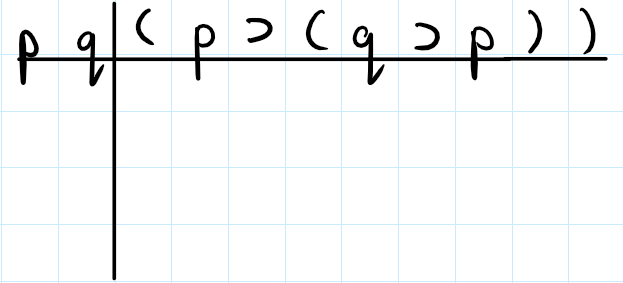
\includegraphics{Pictures/Week4Picture1.png}
If instead, you have the formula \(((r \lor w) \& (\sim j \supset u))\), then you will start your table as follows:

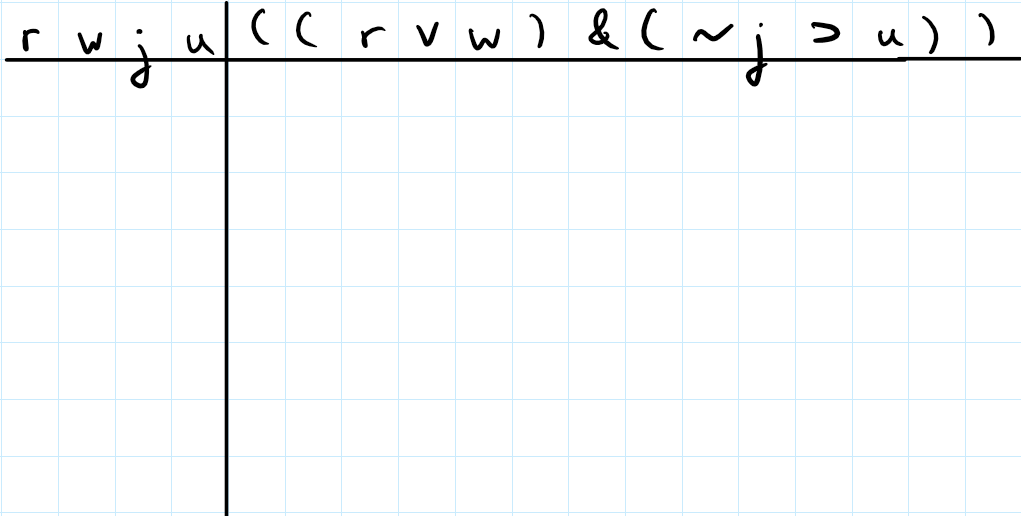
\includegraphics{Pictures/Week4Picture2.png}
3. Next, you fill out the columns for the propositional letters on the left hand side. To do this, you follow a pattern.

First, you determine the number of rows that you need to fill out. For \(n\) different propositional letters, you will have \(2^n\) rows. For example, if you have \(2\) propositional letters, then you will have \(2^2 = 4\) rows. If you have \(3\) propositional letters, then you will have \(2^3 = 8\) rows.

Secondly, starting from the right most propositional letter, you fill out the column by alternating 0s and 1s for each row (this is where figuring out how many rows there are comes in handy; for example, if you know that there will be \(8\) rows, then you will alternate until you have filled out all \(8\) rows). Then you move to the propositional letter one column to the left and you alternate 00 and 11 down the column (you will stop here if you only have two propositional letters). Here is an example:

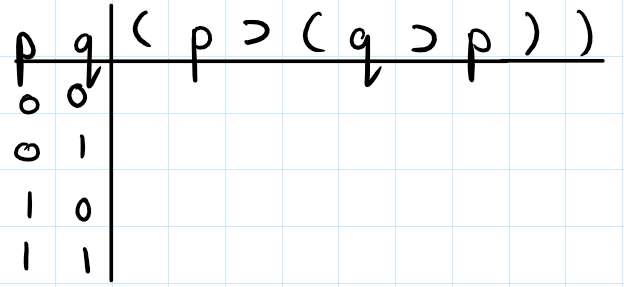
\includegraphics{Pictures/Week4Picture3.png}

If you have more than two propositional letters, move one column to the left and you alternate 0000 and 1111 down the column (you will stop here if you only have three propositional letters). Here is an example:

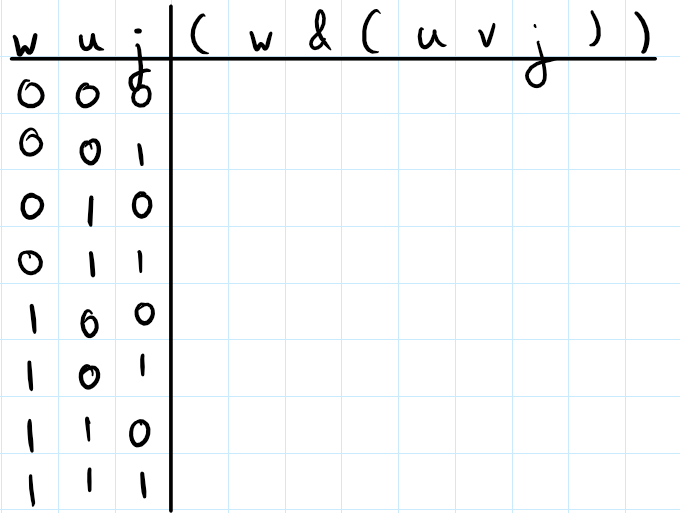
\includegraphics{Pictures/Week4Picture4.png}

If you have more than three propositional letters, then move one column to the left and you alternate 00000000 and 11111111 down the column (you will stop here if you only have four propositional letters). I leave it to you to continue the pattern.

\begin{enumerate}
\def\labelenumi{\arabic{enumi}.}
\setcounter{enumi}{3}
\tightlist
\item
  Now, you can start filling out the columns under the formula that you are concerned with. My advice is to just fill out whatever columns you \emph{can} fill out. This will require you to know how the formulas compose together to form bigger formulas. Here is an example (slightly different from the one I covered in person, in discussion): consider the formula \((p \lor j) \& (\sim p \supset \sim (j \equiv p))\). We start off the table as follows:
\end{enumerate}

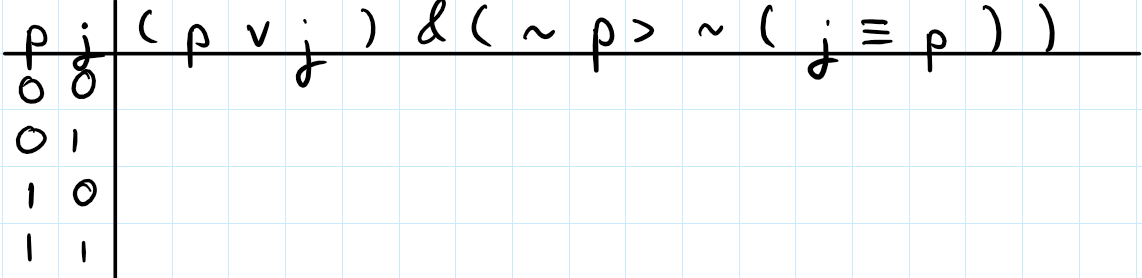
\includegraphics{Pictures/Week4Picture5.png}
Now, we look at the propositional connectives and see which ones we can start to evaluate. Let us consider the \(\&\) connective. Can we evaluate that one yet? Well, we could only evaluate the \(\&\) if we knew the truth value columns of the two formulas that it binds. In this case, the \(\&\) binds together the \((p \lor j)\) and the \((\sim p \supset \sim (j \equiv p))\). Do we currently know what the truth value columns for those formulas are? No.~The truth value column of \((p\lor j)\) would be the column under the \(\lor\) as the \(\lor\) binds together the \(p\) and the \(j\) to create \((p \lor j)\). Can we figure it out? Yes, since we already have the truth value columns for \(p\) and \(j\):

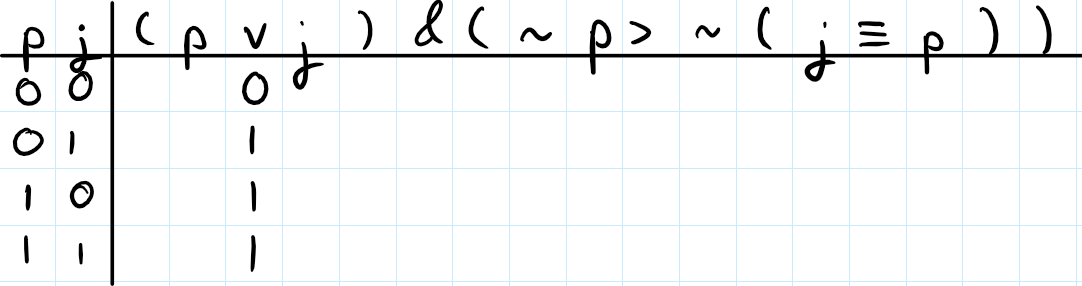
\includegraphics{Pictures/Week4Picture6.png}
So, the left conjunct of the \(\&\) is taken care of. We now need to find the truth value column of the right conjunct. In this case, the column is the one under the \(\supset\) symbol. This is because to form \((\sim p \supset \sim (j \equiv p))\), the \(\supset\) symbol binds together the \(\sim p\) and the \(\sim (j \equiv p)\) formulas. Do we have the truth values of \(\sim p\) and \(\sim (j \equiv p)\)? No.~Can we figure it out? Well, we can quickly fill out the \(\sim p\) since we know the truth value column of \(p\):

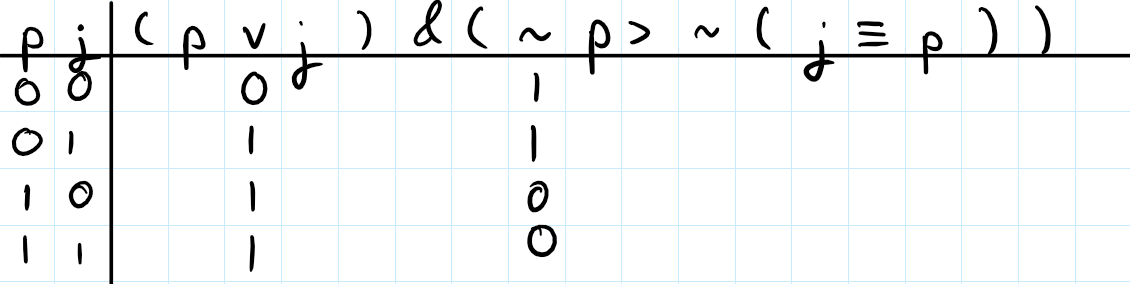
\includegraphics{Pictures/Week4Picture7.png}

Can we do this for \(\sim (j \equiv p)\)? No.~To determine the truth value column under the \(\sim\), we need to first know the truth value column under the \(\equiv\) in \((j \equiv p)\). Thankfully, we can find that since we already have the truth values of \(j\) and \(p\):

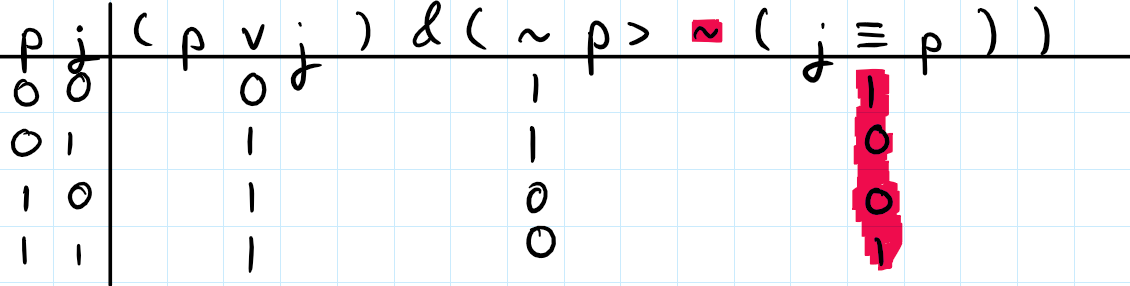
\includegraphics{Pictures/Week4Picture8.png}

Now, we can figure out the truth value column under the \(\sim\). I have highlighted in magenta-red(?), the column that the negation \(\sim\) operates over:

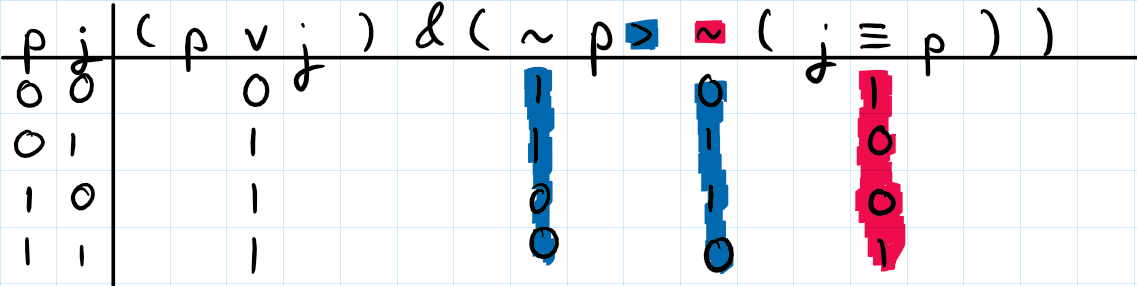
\includegraphics{Pictures/Week4Picture9.png}

Now, remember that the \(\supset\) binded together the \(\sim p\) formula and the \(\sim (j \equiv p)\). The blue highlighted columns are the truth value columns for those formulas and we have both of them now. So we can evaluate the conditional:

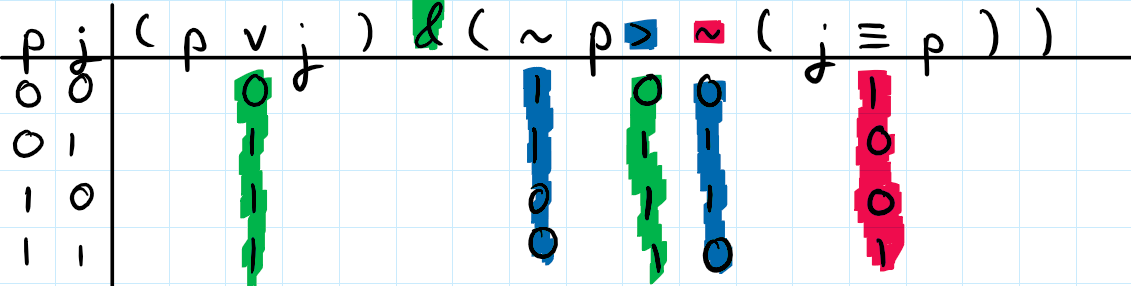
\includegraphics{Pictures/Week4Picture10.png}

Finally, remember that the \(\&\) binded together the \((p \lor j)\) formula and the \((\sim p \supset \sim (j \equiv p))\) formula. The highlighted green columns are the truth value columns for those two formulas. Hence, we can now evaluate the \(\&\), which I will highlight in yellow:

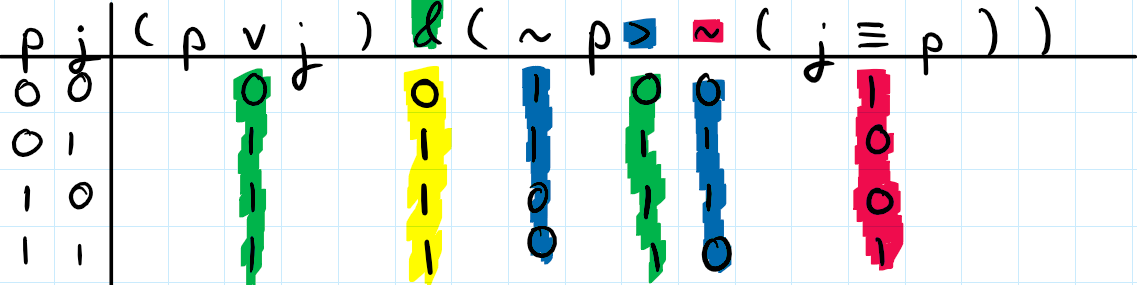
\includegraphics{Pictures/Week4Picture11.png}

That yellow column is the truth value column for the entire formula.

\hypertarget{definitions-of-tautology-contradiction-and-contingency}{%
\section{Definitions of Tautology, Contradiction and Contingency}\label{definitions-of-tautology-contradiction-and-contingency}}

The concepts of tautology, contradiction, and contingency are really important in logic. Sometimes, just by looking at a formula you may be able to tell whether or not it is a tautology, contradiction or contingency, but sometimes you will not be able to. Thankfully, truth tables are one way to always tell whether or not a formula is one of these three.

So, given a formula, to ascertain whether or not it is a tautology, contradiction or a contingency, you:

\begin{enumerate}
\def\labelenumi{\arabic{enumi}.}
\tightlist
\item
  Fill out its truth table.
\item
  Look at the truth value column for the formula that you are concerned with. If the column is all 1s then it is a \emph{tautology}. If the column is all 0s then its a \emph{contradiction}. If the column includes at least one 1 and at least one 0 then it is a \emph{contingency}.
\end{enumerate}

That is all there is to it. Informally, a tautology is a formula which is always true; a contradiction is a formula which is always false; and a contingency is a formula which is sometimes true and sometimes false.

\hypertarget{checking-validity-of-arguments-with-a-truth-table}{%
\section{Checking Validity of Arguments with a Truth Table}\label{checking-validity-of-arguments-with-a-truth-table}}

Sometimes you will be asked to check the validity of an argument using a truth table. The question will often look like ``is \(\phi_1,\phi_2,\ldots,\phi_n \therefore \psi\) valid?'' (the \(\phi_1,\phi_2,\ldots,\phi_n,\psi\) just stand for arbitrary formulas). The formulas before the \(\therefore\) are the premises and the formula after the \(\therefore\) is the conclusion. The procedure for answering such questions is an extension of how to fill out the truth table of a given formula:

\begin{enumerate}
\def\labelenumi{\arabic{enumi}.}
\tightlist
\item
  First look across all the formulas \(\phi_1,\phi_2,\ldots,\phi_n, \psi\) and look at all the distinct propositional letters in those formulas. Start off the left hand side of your truth table with those propositional letters (this is just like the first step for ``How to Fill out a Truth Table''; the only exception is now you are looking at letters across multiple formulas). Next, put the premises \(\phi_1,\ldots,\phi_n,\psi\) to the right of the propositional letters with a line in between each of them. You will end up with something looking like:
\end{enumerate}

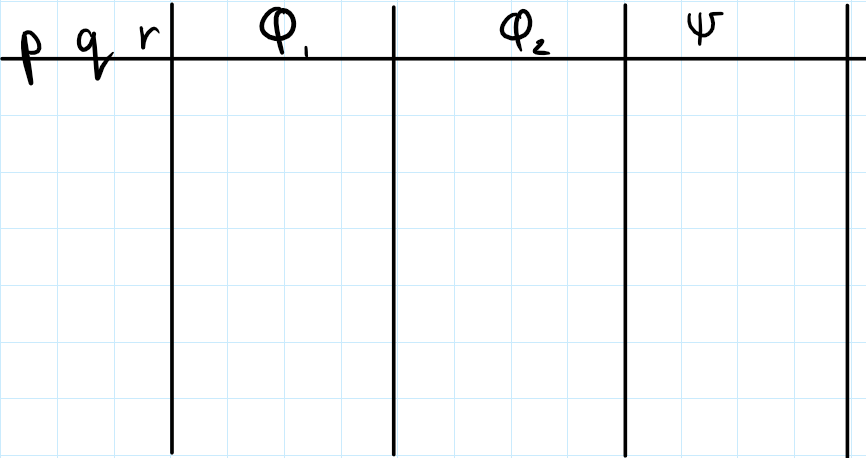
\includegraphics{Pictures/Week4Picture12.png}
(This is a case with two premises \(\phi_1\), \(\phi_2\) and the conclusion \(\psi\)). Next, you fill out the columns for the propositional letters on the left-hand side of the table as you would normally (as in, do the same as step 3. for ``How to Fill Out a Truth Table'').

\begin{enumerate}
\def\labelenumi{\arabic{enumi}.}
\setcounter{enumi}{1}
\item
  Then, working with only one formula at a time, fill out the truth table. For example, if you are working on \(\phi_1\), then you just fill out that truth table; you do not need to consider the other formulas at all. You should end up with truth value columns for all of the formulas (i.e., the premises and the conclusion).
\item
  To evaluate validity, start from the top row and see whether or not it is a row in which the truth value of every premise is a 1. If it is a row in which all the premises are 1, then check whether or not the conclusion is also a 1. If it is \emph{not}, then the argument is invalid and you can stop checking. If it is a 1 then you move onto the row below and repeat the checking procedure. If there is no row below, then you are done and the argument is valid.
\end{enumerate}

\hypertarget{practice-problems-1}{%
\section{Practice Problems}\label{practice-problems-1}}

Provide the truth table for the following (I omit A3, since it is too easy):

\begin{itemize}
\tightlist
\item
  (A1) \((p \lor q) \lor r\)
\item
  (A2) \(\sim (p \& q)\)
\item
  (A4) \((\sim p \lor \sim q)\)
\item
  (A5) \(((p \supset q) \equiv (\sim p \lor q))\)
\end{itemize}

Is the following formula a tautology, contradiction or a contingency? Use a truth table to evaluate:

\begin{itemize}
\tightlist
\item
  (B1) \((p \supset p)\)
\item
  (B2) \((p \supset \sim\sim p)\)
\item
  (B3) \((p \& q) \lor (q \& p)\)
\item
  (B4) \(\sim (p \supset (q \supset p))\)
\item
  (B5) \(((q \supset p) \supset (\sim q \supset \sim p))\)
\item
  (B6) \(((p \supset ((p \supset q) \equiv (p \& \sim r))) \lor r)\)
\end{itemize}

Which of the following arguments are valid?

\begin{itemize}
\tightlist
\item
  (C1) \((\sim p \lor q), q \therefore \sim p\)
\item
  (C2) \((\sim p \supset (q \lor p)), \sim p \therefore q\)
\item
  (C3) \((p \equiv (q \& \sim p)), (q\supset p) \therefore (q \lor p)\)
\end{itemize}

\hypertarget{solutions}{%
\section{Solutions}\label{solutions}}

Under the main column you should have (left-to-right = top-to-bottom)

\begin{itemize}
\tightlist
\item
  (A1) \(01111111\)
\item
  (A2) \(1110\)
\item
  (A4) \(1110\)
\item
  (A5) \(1111\)
\end{itemize}

Then for the other questions, I just give the answers you should arrive at (I also quickly did these so there is a possibility of a mistake):

\begin{itemize}
\tightlist
\item
  (B1) Tautology
\item
  (B2) Tautology
\item
  (B3) Contingency
\item
  (B4) Contradiction
\item
  (B5) Tautology
\item
  (B6) Contingency
\item
  (C1) Invalid
\item
  (C2) Valid
\item
  (C3) Invalid
\end{itemize}

  \bibliography{book.bib,packages.bib}

\end{document}
